% to sort

% need plane direct diagram inkscape
% sphere coord needs middlie red line to get slice count consistent
% torus diagram needs colour
% fig refs not working ?
% degenerate points
% subtraction and addition of booleans
% bdsim shooting particles at geant4 sphere and then new old mesh with incresing desities
% then bdsim of compound solids
% hyperboiloid poly count still needs to be done
% mention wether software are free ?
% cylindrical image has random theta
% backwards quotation marks
% polygon count also counts triangles 
% equations for motion of a particle
% need to have local copy of code if it changes
% figures should pdfs
% polycone stack kept at 3

\documentclass[12pt,a4paper]{article}
\usepackage{graphicx}
\usepackage{hyperref}   
\usepackage{braket}
\usepackage{amsmath}

\usepackage[utf8]{inputenc}
\usepackage[english]{babel}

\usepackage{listings}
\usepackage{color}
\usepackage[margin=0.75in]{geometry}
\usepackage{subfigure}

\definecolor{mygreen}{rgb}{0,0.6,0}
\definecolor{mygray}{rgb}{0.5,0.5,0.5}
\definecolor{mymauve}{rgb}{0.58,0,0.82}
\usepackage{afterpage}

\newcommand{\ts}{\textsuperscript}
\usepackage[super]{nth}
\usepackage{gensymb}
\usepackage{xcolor}
\usepackage{wasysym}
%\usepackage{wasysym} %for astro symbols

 \lstset{ 
  backgroundcolor=\color{white},  % choose the background color; you must add \usepackage{color} or \usepackage{xcolor}; should come as last argument
  basicstyle=\footnotesize,             % the size of the fonts that are used for the code
  breakatwhitespace=false,            % sets if automatic breaks should only happen at whitespace
  breaklines=true,                          % sets automatic line breaking
  captionpos=b,                             % sets the caption-position to bottom
  commentstyle=\color{mygreen},   % comment style
  deletekeywords={...},                   % if you want to delete keywords from the given language
  escapeinside={\%*}{*)},             % if you want to add LaTeX within your code
  extendedchars=true,                    % lets you use non-ASCII characters; for 8-bits encodings only, does not work with UTF-8
  frame=single,	                            % adds a frame around the code
  keepspaces=true,                         % keeps spaces in text, useful for keeping indentation of code (possibly needs columns=flexible)
  keywordstyle=\color{blue},            % keyword style
  language=Octave,                         % the language of the code
  morekeywords={*,...},                  % if you want to add more keywords to the set
  numbers=left,                               % where to put the line-numbers; possible values are (none, left, right)
  numbersep=5pt,                            % how far the line-numbers are from the code
  numberstyle=\tiny\color{mygray},   % the style that is used for the line-numbers
  rulecolor=\color{black},                 % if not set, the frame-color may be changed on line-breaks within not-black text (e.g. comments (green here))
  showspaces=false,                        % show spaces everywhere adding particular underscores; it overrides 'showstringspaces'
  showstringspaces=false,               % underline spaces within strings only
  showtabs=false,                           % show tabs within strings adding particular underscores
  stepnumber=2,                             % the step between two line-numbers. If it's 1, each line will be numbered
  stringstyle=\color{mymauve},        % string literal style
  tabsize=2,	                             % sets default tabsize to 2 spaces
  title=\lstname                               % show the filename of files included with \lstinputlisting; also try caption instead of title
} 

\usepackage{multicol}
\usepackage[font=small,labelfont=bf]{caption} % Makes the font for figure captions smaller and the figure label bold.

\begin{document}
%\pagecolor{black}\afterpage{\nopagecolor}
%\color{white}
\begin{titlepage}
	\centering
	
\includegraphics[width=0.4\textwidth]{Images//Logos//rhul.jpg}\par\vspace{1cm}


	{\scshape\LARGE Royal Holloway University of London \par}
	\vspace{1cm}
	{\scshape\Large PH4100: Major Project\par}
	\vspace{1.5cm}
	{\huge\bfseries Meshing of Primitive Solids\\
	in\\
	pyg4ometry \& BDSIM\par}
	\vspace{2cm}
	{\Large\itshape Ben Shellswell\par}
	\vfill

\begin{abstract}
\centering

\end{abstract}
When testing new concepts and devices within particle physics it is often a very expensive and time consuming process. The software packages pyg4ometry \& BDSIM are designed to enable scientists and people within in the industry to virtually simulate these tests, with accurate physics concepts. This project looks at improving the 3D simulation of the events and devices, by remeshing the basic primitive solids.

	\vfill
	
	Supervised by\par
	Prof.~S \textsc{Boogert} 

% Bottom of the page
	{\large \today\par}



\begin{figure}[h]
\centering
\begin{minipage}{.6\textwidth}
  
\includegraphics[width=0.4\textwidth]{Images//Logos//BDSIM_Logo.jpg}
\end{minipage}%
\begin{minipage}{.6\textwidth}
  \centering
  
\includegraphics[width=0.5\textwidth]{Images//Logos//JAI_Logo.jpeg}
  \end{minipage}
\end{figure}

\end{titlepage}
\leavevmode\thispagestyle{empty}\newpage
%\color{black}
\tableofcontents
\thispagestyle{empty}
\newpage
\onecolumn

%%%%%%%%%%%%%%%%%%%%%%%%%%%%%%%%%%%%%%%%%%%%%%%%%%%%%%%%%%%%%%%%%%%%%%
\small
\setcounter{page}{1}

% ------------------------------------------------------------------------------------------------------------------------------

\section{Introduction}

\subsection{Project Aims}
The aims of this project are to contribute towards the optimization of the pyg4ometry package \ref{pyg} (and subsequently BDSIM \ref{bdsim}), by improving parts of the code and conducting performance test to produce results that can be analysed. The main areas for improvement and where most of the computational energy in wasted, is in the meshing of the primitive Geant4 \ref{g4} compatible solids, due to the unessecary use of boolean operations \ref{bool}.

\subsection{Report Structure}
The subsequent sections are constructed in the following way, the software packages that are used and referenced through out this report (Section \ref{packs}), the concept and details of the primitive meshing used in pyg4ometry (Section \ref{prim}), then a conclusion and summary of the results of the report (Section \ref{conc}).


% ------------------------------------------------------------------------------------------------------------------------------

\section{Software Packages}
\label{packs}
This section goes through each package of software related to and used throughout the duration of the project. It outlines the key details of each package, describing its function and link to the project.

\subsection{BDSIM}
\label{bdsim}
BDSIM (or Beam Delivery SIMulation) is a open source software package written by the John Adams Institute (JAI) \cite{jai}, for the use of modelling particle beam interactions. BDSIM has many applications, such as modelling complex particle accelerators for example the Large Hadron Collider (LHC) or concepts magnets for medical scanners used to treat tumors. The package allows a user to specify the physics being used for a particular particle of a set energy colliding with a provided object. The scattering of the particle trajectories and decays are computed using monte carlo simulations, to make the results as consistent with experimental results as possible. The software outputs a full analysis of each run, and can even allow multiple runs to run at once (batch mode).

\subsection{pyg4ometry}
\label{pyg}
pyg4ometry is an open source python package also generated by JAI, its purpose is to convert 3D CAD (Computer Aided Design) models between different representations to allow compatibility with BDSIM for the testing of new concepts. The '4' in 'pyg4ometry' comes from the consistencey the package has with Geant4 \ref{geant4}. The package is a key tool for allowing multiple file formats to become compatible with BDSIM, which increases the number of people who can utilise the package.

\subsection{Geant4}\label{geant4}
\label{g4}
Geant4 (or GEometry ANd Tracking) is a software developed for the simulation and tracking of particles traveling through matter.



% ------------------------------------------------------------------------------------------------------------------------------
\newpage
\section{Primitive Meshing}
\label{prim}
This section will describe the work done to optimize the python scripts that generate the three dimensional meshing for the primitive solids within the pyg4ometry package \ref{pyg}. All the primitive solids used are constructed such that they are compatible with Geant4's solids. It was orginally thought that it would be best to use trianglar based meshes in combination with boolean operations \ref{bool} to construct the 3D solids. However it has been realised that the computation of triangles and boolean operations compared with polygons and adapted trigonometry is much more intensive and ineffecient, in most cases. In particular with the curved solids, i.e circular and elliptical based solids.
\\\\
One of the major improvements to the pyg4ometry \ref{pyg} code is the computation of cut up primitive solids. The meshing of hollow or sliced solids were previously computed by Boolean subtractions and unions, which involved creating two separate solids and acting upon both of them. Discussed more in Section \ref{bool}. Which resulted in a very computationally heavy and less aestetic outcome, where the mesh lines ('slice and stack'), were not meshed in radial directions.

\subsection{Co-ordinate Systems}
The various primitive solids are all constructed by using the predefined parameters used by Geant4 \ref{g4}, to be consistent with Geant4's own solids. The parameters of a 3D solid are properties relating to the coordinate system it is constructed in, such as height or radius. The parameters are then used to define the points of the object via basic trigonometry.
\\\\
The python meshing scripts for all coordinate systems follow a similar structure, of first defining an empty list of faces (polygons). Then running the associated trigonometric equations through a number of loops to generate and append polygons to that list. The number of loops is associated with the number of sections a surface of a solid is being split up into in a given coordinate system. The density of the meshing is defined by a user inputted number of slices and stacks, demonstrated in Figure \ref{cylcmeshin}.

\subsubsection{Cylindrical Co-ordinate System}
\label{cycl}
The meshing for the primitive solids in cylindrical polar coordinate systems are constructed by looping though the user defined number of slices and stacks (as shown in Figure \ref{cycmeshin}) which the cylinder is being cut into (Listing \ref{code1}). The Loop then creates the coordinates for 3 or 4 points at a time using an adapation to the trigonometry in Equations \ref{cyctrig}, which can then be defined as a triangular or polygonal face. The only cases where the mesh produces triangles is at the top and bottom faces of the cylinder, provided it does has a minimum radius equal to zero (creating a tube or cone). The same logic for the polygons also applied to triangles, just using 3 vertex points to make a face.

\begin{figure}[h!]
\centering
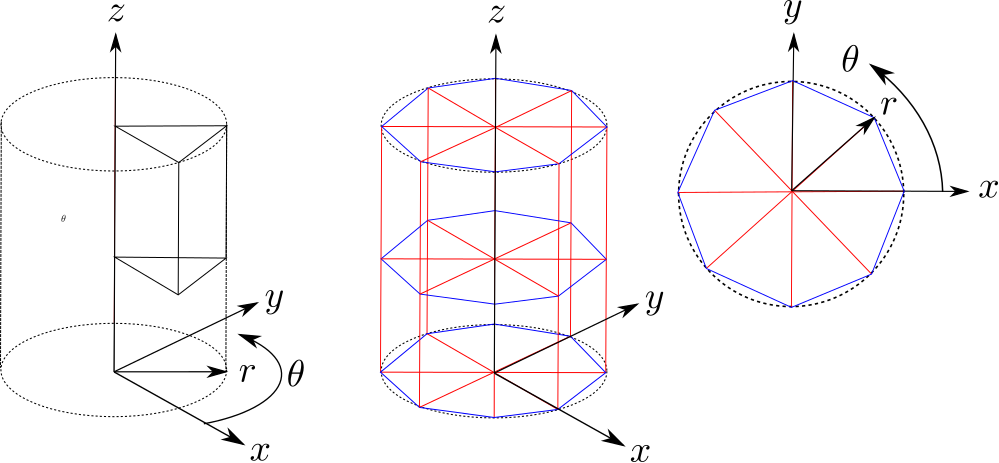
\includegraphics[scale=0.45]{Images//Coords//cyl.png}
\caption[width=\columnwidth]{Diagram showing the meshing method for a cylindrical coordinate system\\
Red = Slices   (8)\\
Blue = Stacks (2)}
\label{cylmeshin}
\end{figure}
\vspace{0.3cm}
The trigonometry that converts the points from cylindrical polar coordinates to cartesian, are:
\begin{equation}
\begin{aligned}
\label{cyctrig}
& x = r \cos{\theta} \\
& y = r \sin{\theta} \\
& z = z
\end{aligned}
\end{equation}

%\label{code1} 
\newpage
\begin{lstlisting}[language=Python, label=code1, caption=Basic method structure for pyg4ometry primitive meshing of solids]
polygons = []

for j0 in range(nslice):
    j1 = j0
    j2 = j0 + 1
    
    vertices = []

    for i0 in range(nstack):
          i1 = i0
          i2 = i0 + 1     

\end{lstlisting}
The code in Listing \ref{code1} generates counters so that you can choses from two slices and two stacks, in order to gain the four points surrounding a desired face. These points are then used to define a polygon. 
\\\\
The only time a stack is needed in the cylindrical coordinate system is when the solid has a non linear function in the r-z plane. For example a paraboild (Figure \ref{para}) would need a stack, but a linear cone (Figure \ref{cons}) would not. This is due to the fact how that a plane can't represent a curved surface with a singe face. 

\newpage
\subsubsection{Spherical Coordinate System}

The meshing for the primitive solids in spherical coordinate systems are constructed by similar means the that of the cylindrical \ref{cycl}. Just with different trigonometric equations (Equations \ref{trigsph}) as a result of two angle parameters $\phi$ and $\theta$. The stack (blue) and slice (red) for solids in the spherical coordinate system works, like the longitude and latitude on a globe, as shown in Figure \ref{sphmeshin}. 
\\\\
The trigonometry that converts the points from spherical coordinates to cartesian, are:

\begin{equation}
\begin{aligned}
& x = r \cos{\theta}\sin{\phi}\\
& y = r \sin{\theta}\sin{\phi} \\
& z = z
\end{aligned}
\label{trigsph}
\end{equation}
\begin{figure}[h!]
\centering
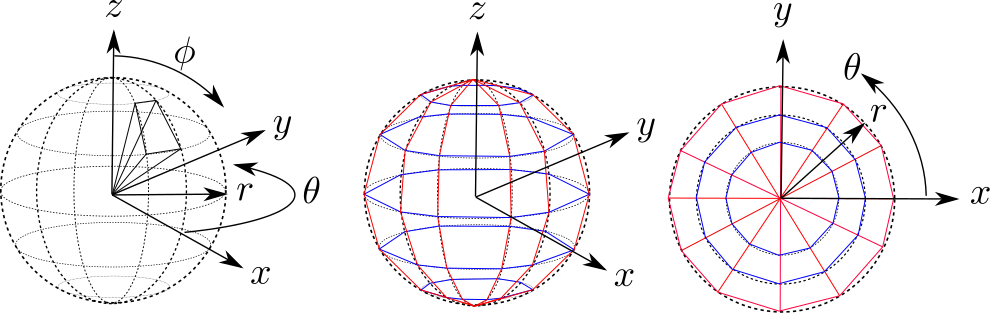
\includegraphics[scale=0.5]{Images//Coords//sph.png}
\caption[width=\columnwidth]{Diagram showing the meshing method for a spherical coordinate system\\
Red = Slices (12)\\
Blue = Stacks (6)}
\label{sphmeshin}
\end{figure}

\noindent The structure of the code is the same as used in Listing \ref{code1}.\\\\
\noindent The only time triangles are constructed in the spherical coordinate system is if the solid has a complete pole at the top or bottom of the solid. The solids constructed in the spherical always have both a stack and a slice.

%\begin{lstlisting}[language=Python, caption=Python example]
%for j0 in range(nslice):
%    j1 = j0
%    j2 = j0 + 1
%
%    for i0 in range(nstack):
%          i1 = i0
%          i2 = i0 + 1
%\end{lstlisting}

\newpage
\subsubsection{Toroidal Coordinate System}

A toridal shape is much harder to visualise a stack and slice, due to the fact it is a rotating coordinate system. A toroidal slice is an $R_{Torus}$ radial cut taken out of the angle $\phi$, as shown in Figure \ref{tormeshin}. The toroidal stack is a $R$ radial cut out of the angle $\theta$. 
\\\\
The trigonometry that converts the points from toroidal coordinates to cartesian, are:

\begin{equation}
\begin{aligned}
& x = R_{Torus} + R\cos{\theta}\cos{\phi} \\
& y = R_{Torus} + R\cos{\theta}\sin{\phi} \\
& z =  R\sin{\theta} 
\end{aligned}
\end{equation}

\begin{figure}[h!]
\centering
\includegraphics[scale=0.35]{Images//Coords/torus_coords.png}
\caption[width=\columnwidth]{Diagram showing the meshing method for a toroidal coordinate system}
\label{tormeshin}
\end{figure}

\subsection{Plane Direction}
One key thing to be taken into account is the convention being used in the code for the order in which points are appended to make a plane, i.e to define a face on a solid. This is important as the direction the normal of the plane points in, dictates wether a face is considered an inside or outside face on the given solid. Getting this incorrect, will lead to missing faces, when the meshing is made. The concept is demonstrated in Figure \ref{pointsorder}.

\begin{figure}[h!]
\centering
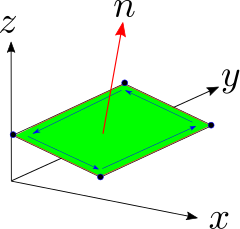
\includegraphics[scale=0.75]{Images//append_points//Point_Appending_Order.png}
\caption[width=\columnwidth]{Diagram showing the order convention of appending points to define the normal to a plane}
\label{pointsorder}
\end{figure}
\noindent The simplest way to test this is by performing boolean operations with a box, as the boolean operation will only work nicely if all the planes are correct on both shapes.

\subsection{New Meshing of Curved Primitve Solids}
In total there are 12 curved primitive solids, of which many of the examples and concepts are very similar. Therefore only a few solids will be discussed in this section, but their development can all be viewed in Appendix \ref{app1}.
\\\\
can give one eaxmple and reference rest in appendix, radial meshing clean up, can remove stack in some cases, boolean slow and messy

\begin{figure}[h!]
\centering
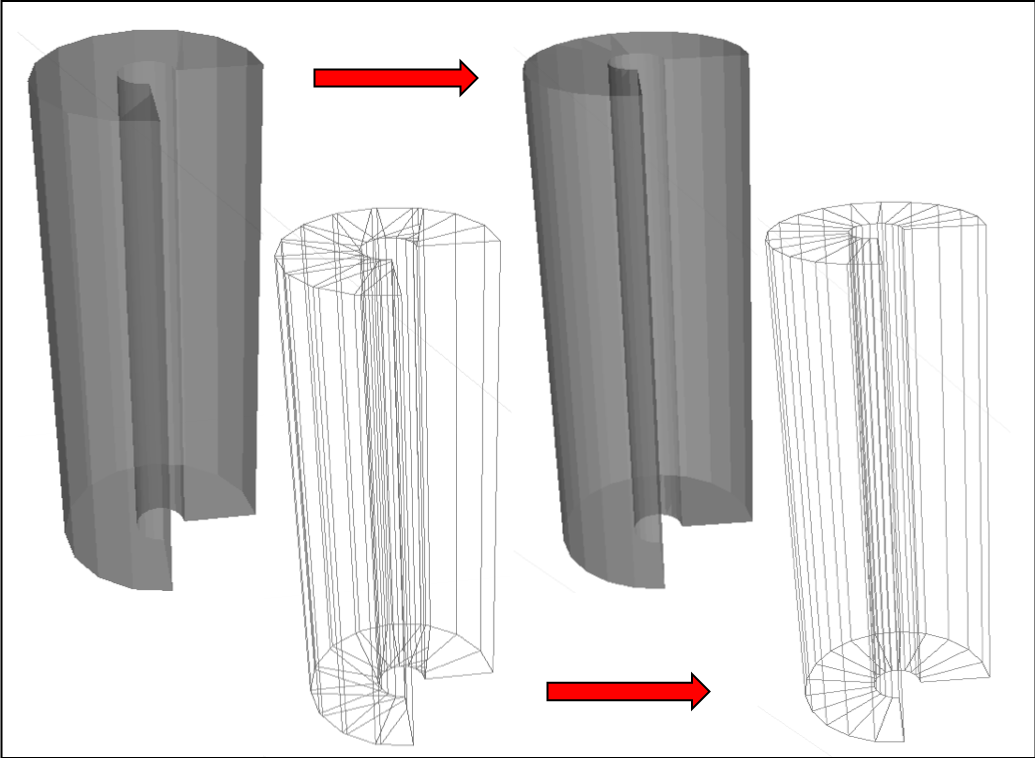
\includegraphics[scale=0.5]{Images//Meshes//tubs.png}
\caption[width=\columnwidth]{Meshing Development for CutTubs (Solid \& Mesh View)}
\label{tubspic}
\end{figure}



\subsubsection{Degenerate points}
Multiple points occupying the same area can spring a few errors with out crashing the code, therefore can sometimes be tricky to spot. 

\subsubsection{Boolean operations}
\label{bool}
One of the largest changes to the performance of the new meshing compared with the previous method, is the disgarding of boolean operations in order to create hollow or cut-up primitive solids. The Old meshing algorithurms would make two solids one smaller that the other and subtract it, with the aim of creating a new shape that is hollow. For example Tubs is made from two cylinders being subtracted in order to create a tube as seen in Figure \ref{tubspic}. The boolean operations worked, however are very computationally heavy compared with that of some adapated trigonometry. Another thing the boolean operations affected was the appearance of the mesh its self, the boolean operations worked by trying to identify common mesh points and then remeshing. This created alot of non radially uniform mesh sections as seen in Tubs.

\begin{figure}[h!]
\centering
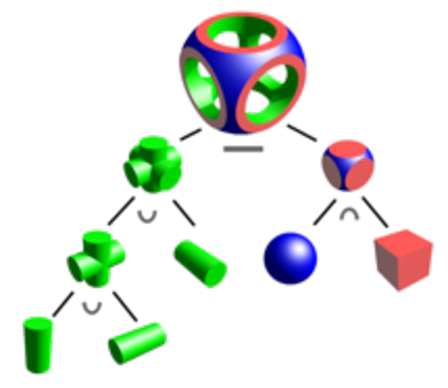
\includegraphics[scale=1]{Images//Booleans//Boolean.pdf}
\caption[width=\columnwidth]{Meshing Development for CutTubs (Solid \& Mesh View)}
\label{tubspic}
\end{figure}

\subsection{Meshing performance testing}
\subsubsection{Polygon Count}

\begin{figure}[h!]
\centering
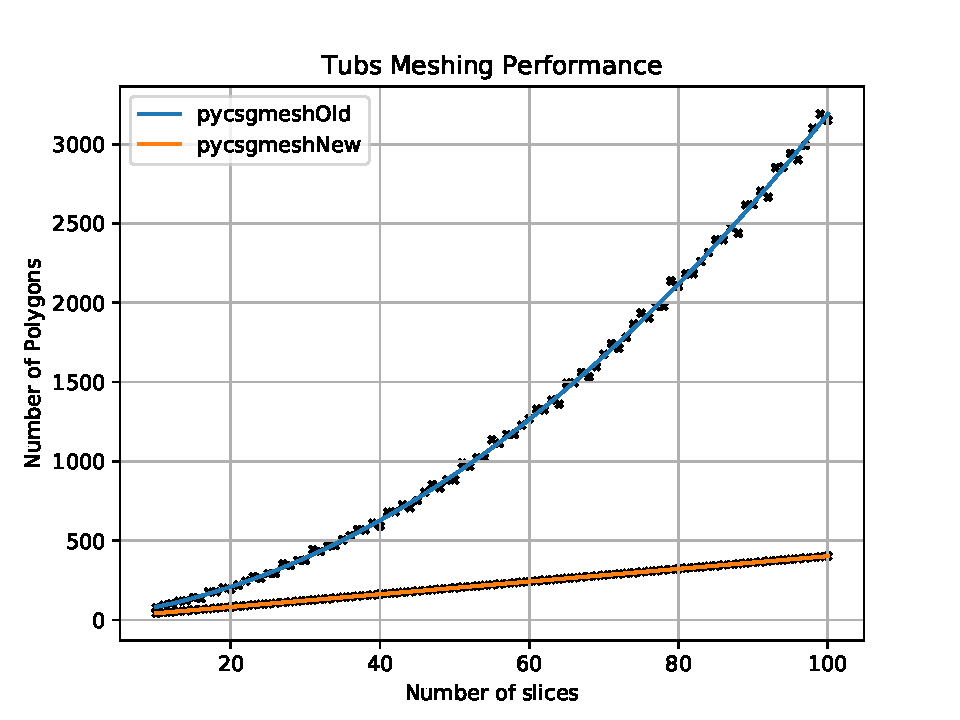
\includegraphics[scale=0.6]{Images//Quad_fits//Tubs_quad.pdf}
\caption[width=\columnwidth]{A plot showing the comparison of the number of polygons (and triangles) generated by the new and old meshing methods, across a range of slice 10-100.}
\label{conts}
\end{figure}
\subsubsection{BDSIM interactions}

\newpage
\section{Conclusion \& Summary}
\label{conc}
\subsection{Improvements}
meshing is quicker\\
improved coverage unit test speeds\\
meshing is neater and more uniform in structure\\
higher meshing density = closer to tru solid as expected with bdsim interactions\\

\subsection{Applications}
BDSIM and pyg4ometry are both very powerful software packages that can be used to to aid not only the scientific research community of particle physicist, but also help everyday people treat patients. Thanks to the software being open source and its wide range of file compatibilities it can be used to simulate a growing number of projects.


% ------------------------------------------------------------------------------------------------------------------------------

\newpage
\appendix

\section{Appendix (Python scripts)}
\subsection{Sphere BDSIM Vary Mesh Test}\label{ap1}
\lstinputlisting[language=Python]{Scripts//Run_New_Meshes.py}

%\newpage
%\subsection{Discovery method contribution pie chart (Figure \ref{pie})}\label{ap2}
%\lstinputlisting[language=Python]{Python//pi.py}

\newpage
\twocolumn[\section{All Meshed Solids and Polygon Count Plots}
\label{app1}
The following Figures are the meshing and polygon data for each primitive solid constructed in pyg4ometry \ref{pyg}. The first Figure for each solid is screenshots of the old meshing and new meshing visualized in VTK. They show the before and after of each primitive solid in both "solid view" and "mesh view". The second Figures Show the number of polygons and triangles produced by the solid as you increase the slice across a range of 10-100 (if there is a stack it is kept at a constant 10). The polygon data plots are generate using python 2.7. The naming convention is the one used by Geant4 \ref{g4}.\\]
\begingroup
\subsubsection{Cons}
\begin{figure}[h!]
\centering
\begin{minipage}{.2\textwidth}
  \centering
  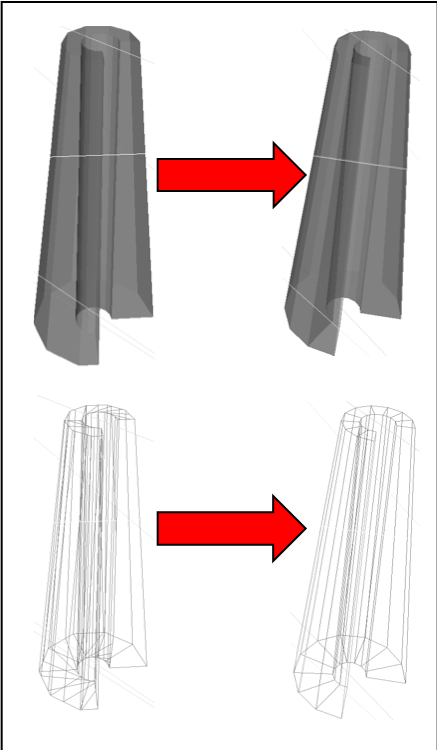
\includegraphics[height=1\linewidth]{Images//Meshes//cons.png}
  \captionof{figure}{}
  \label{fig:test1}
\end{minipage}%
\begin{minipage}{.3\textwidth}
  \centering
  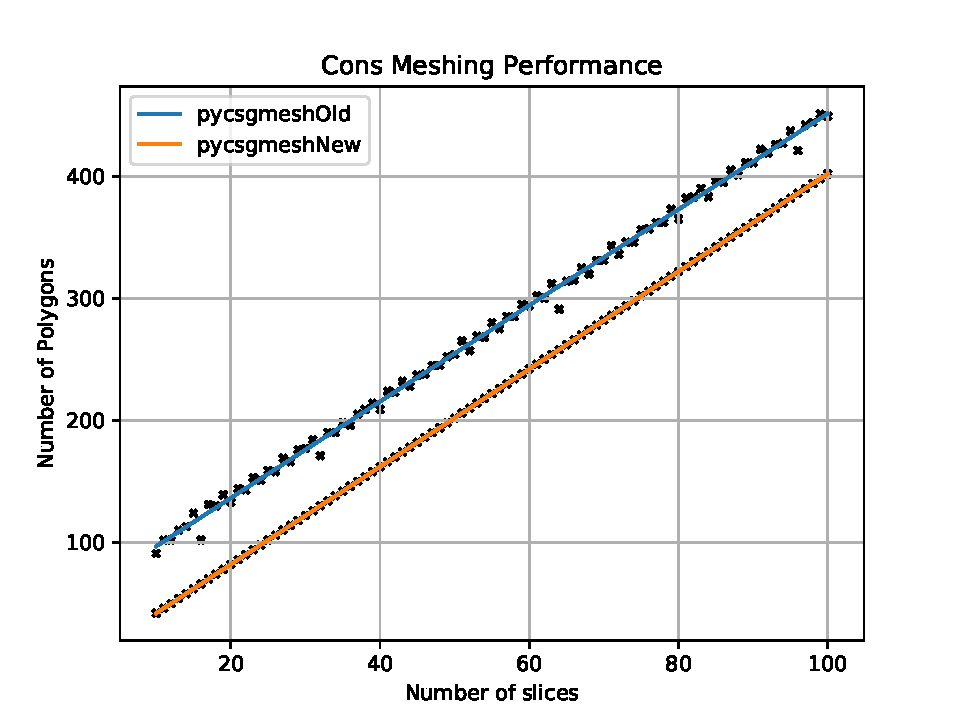
\includegraphics[scale=0.35]{Images//Quad_fits//Cons_quad.pdf}
  \captionof{figure}{ }
  \label{fig:test2}
\end{minipage}%
\end{figure}

\subsubsection{CutTubs}

\begin{figure}[h!]
\centering
\begin{minipage}{.2\textwidth}
  \centering
  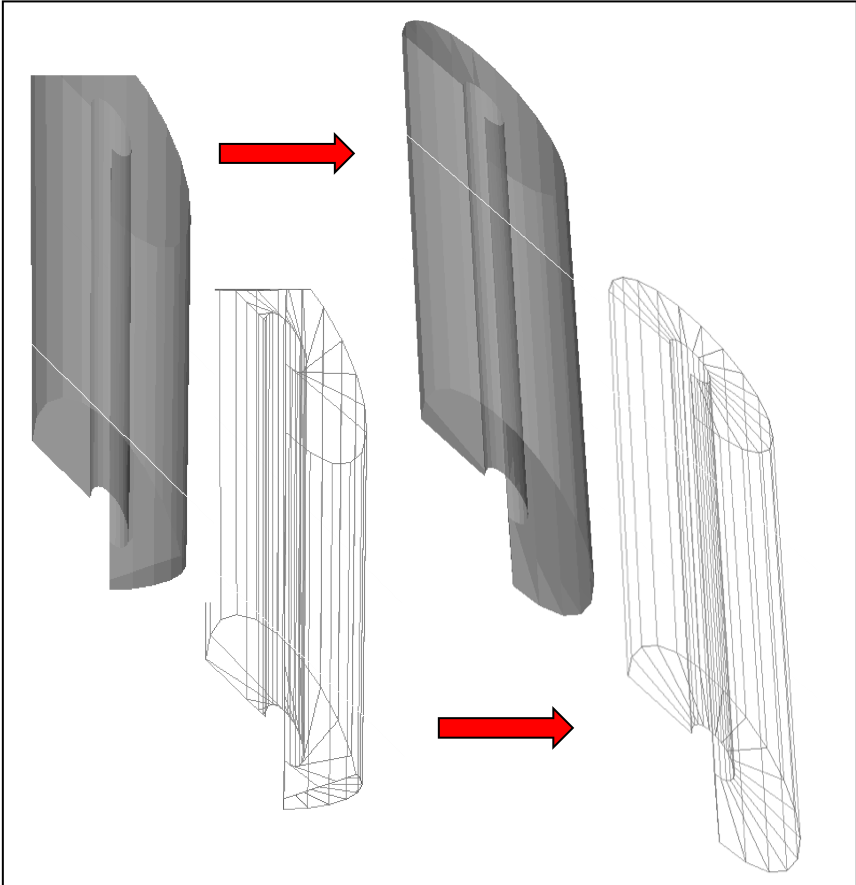
\includegraphics[height=1\linewidth]{Images//Meshes//CutTubs.png}
  \captionof{figure}{ }
  \label{fig:test1}
\end{minipage}%
\begin{minipage}{.3\textwidth}
  \centering
  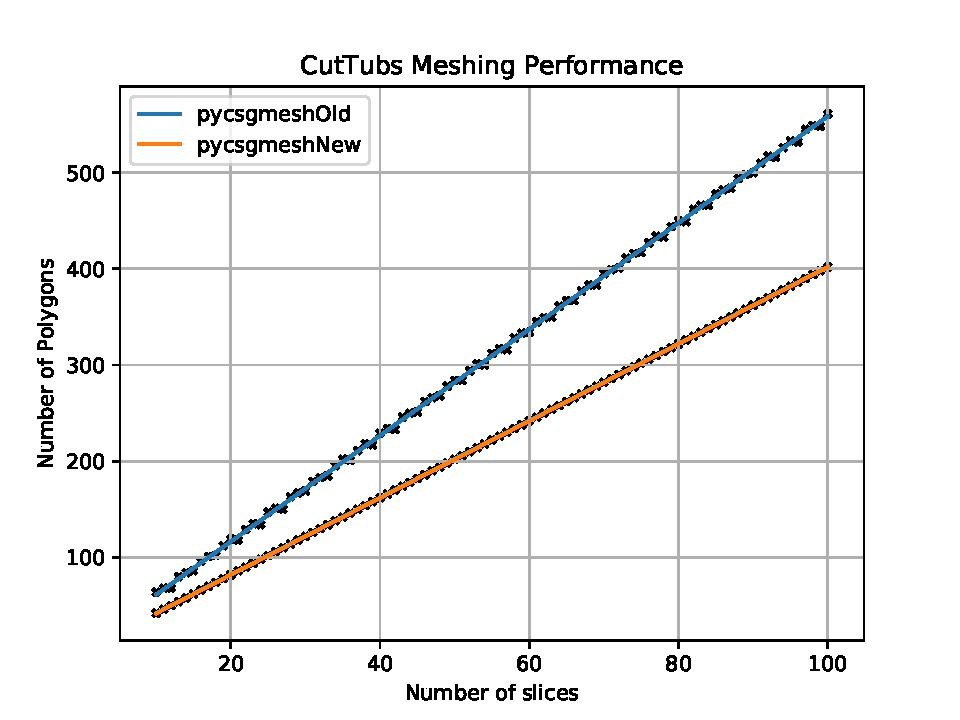
\includegraphics[scale=0.35]{Images//Quad_fits//CutTubs_quad.pdf}
  \captionof{figure}{ }
  \label{fig:test2}
\end{minipage}%
\end{figure}

\subsubsection{Ellipsoid}

\begin{figure}[h!]
\centering
\begin{minipage}{.2\textwidth}
  \centering
  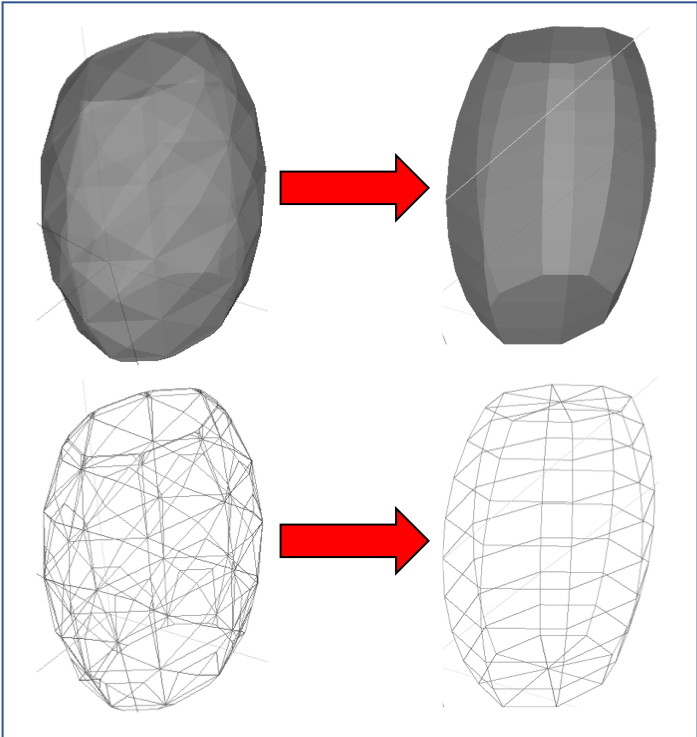
\includegraphics[height=1\linewidth]{Images//Meshes//ellipsoid.png}
  \captionof{figure}{ }
  \label{fig:test1}
\end{minipage}%
\begin{minipage}{.3\textwidth}
  \centering
  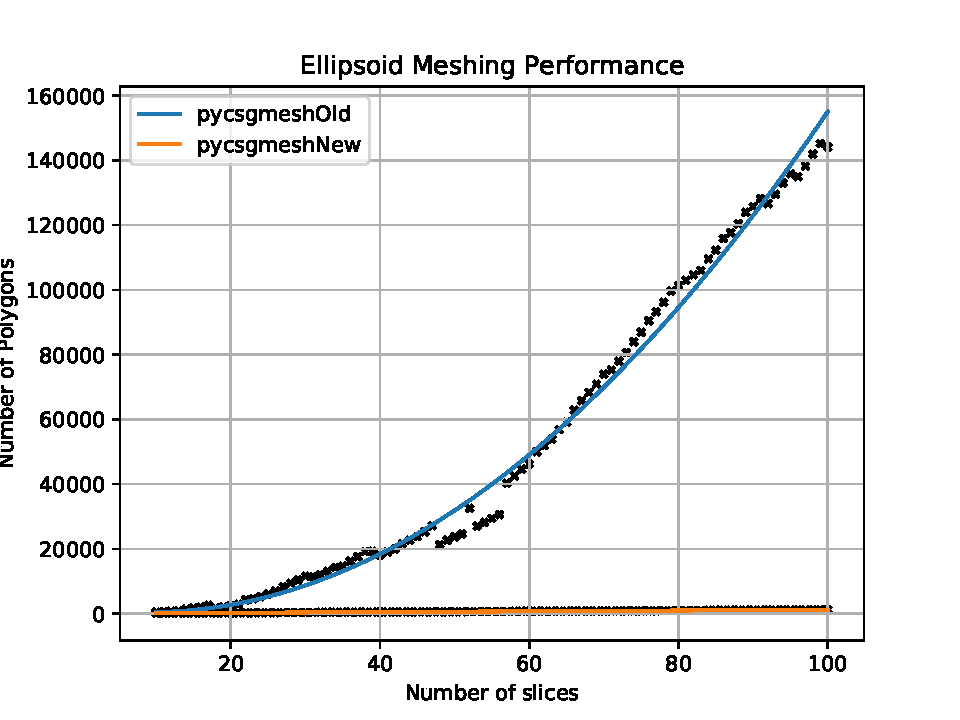
\includegraphics[scale=0.35]{Images//Quad_fits//Ellipsoid_quad.pdf}
  \captionof{figure}{ }
  \label{fig:test2}
\end{minipage}%
\end{figure}

\newpage
\subsubsection{EllipticalCone}

\begin{figure}[h!]
\centering
\begin{minipage}{.2\textwidth}
  \centering
  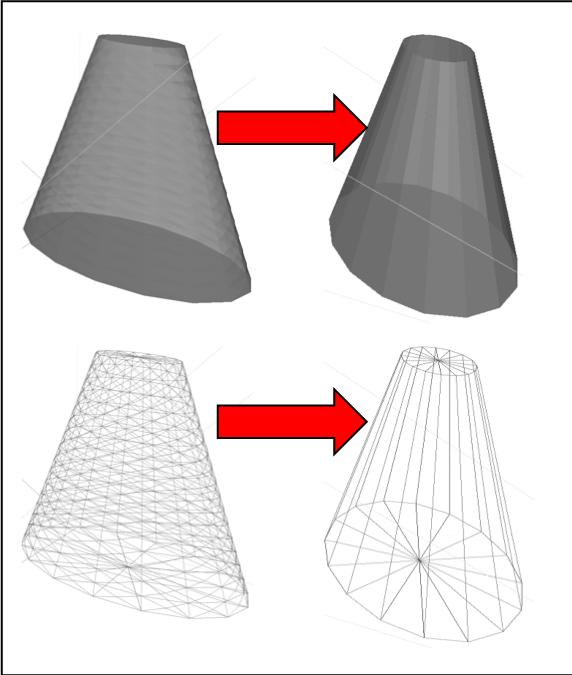
\includegraphics[height=1\linewidth]{Images//Meshes//ellipticalcone.png}
  \captionof{figure}{ }
  \label{fig:test1}
\end{minipage}%
\begin{minipage}{.3\textwidth}
  \centering
  \includegraphics[scale=0.35]{Images//Quad_fits//Ellipticalcone_quad.pdf}
  \captionof{figure}{ }
  \label{fig:test2}
\end{minipage}%
\end{figure}

\subsubsection{EllipticalTube}

\begin{figure}[h!]
\centering
\begin{minipage}{.2\textwidth}
  \centering
  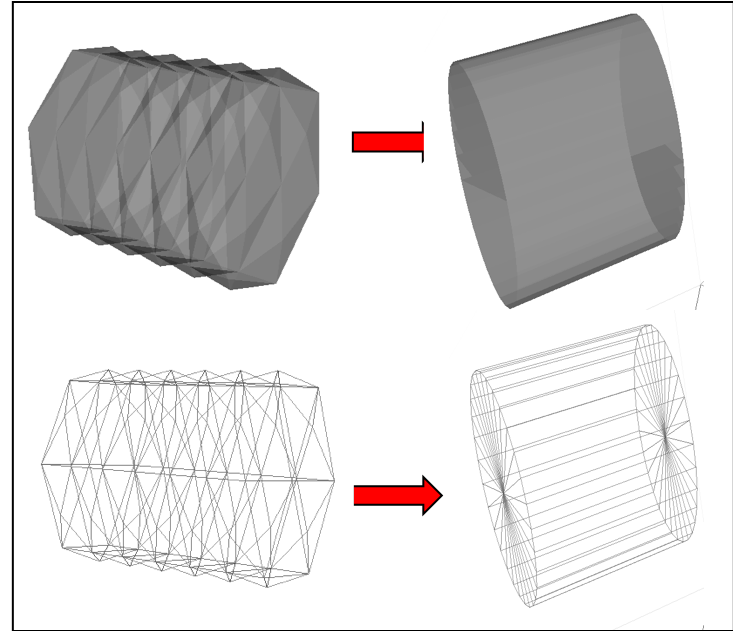
\includegraphics[height=0.8\linewidth]{Images//Meshes//ellipticaltube.png}
  \captionof{figure}{ }
  \label{fig:test1}
\end{minipage}%
\begin{minipage}{.3\textwidth}
  \centering
  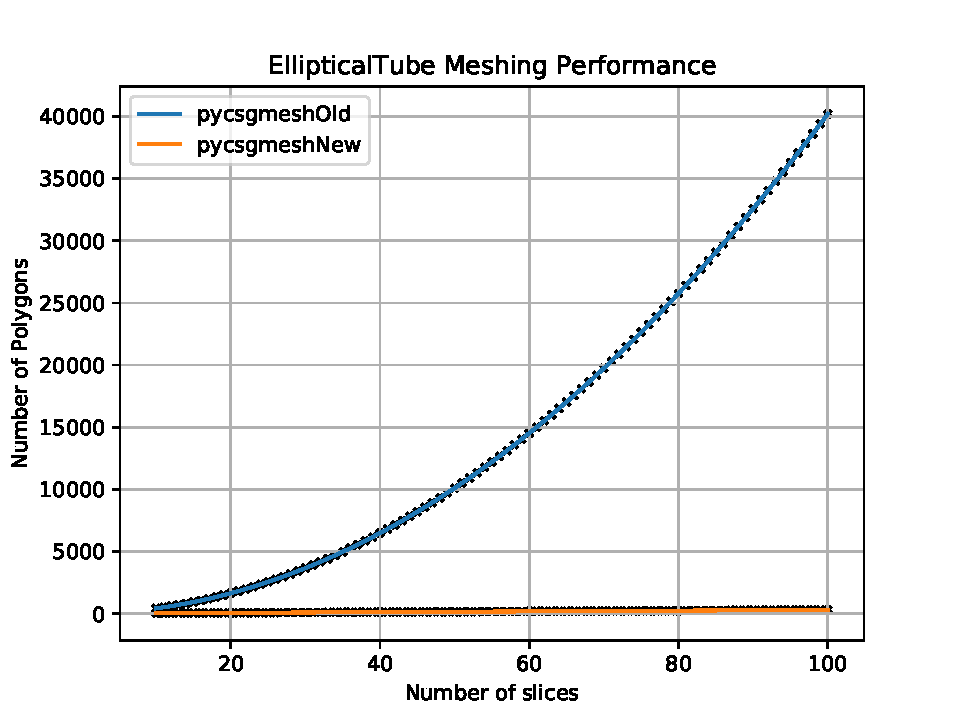
\includegraphics[scale=0.35]{Images//Quad_fits//EllipticalTube_quad.pdf}
  \captionof{figure}{ }
  \label{fig:test2}
\end{minipage}%
\end{figure}

\subsubsection{Hyperboloid}

\begin{figure}[h!]
\centering
\begin{minipage}{.2\textwidth}
  \centering
  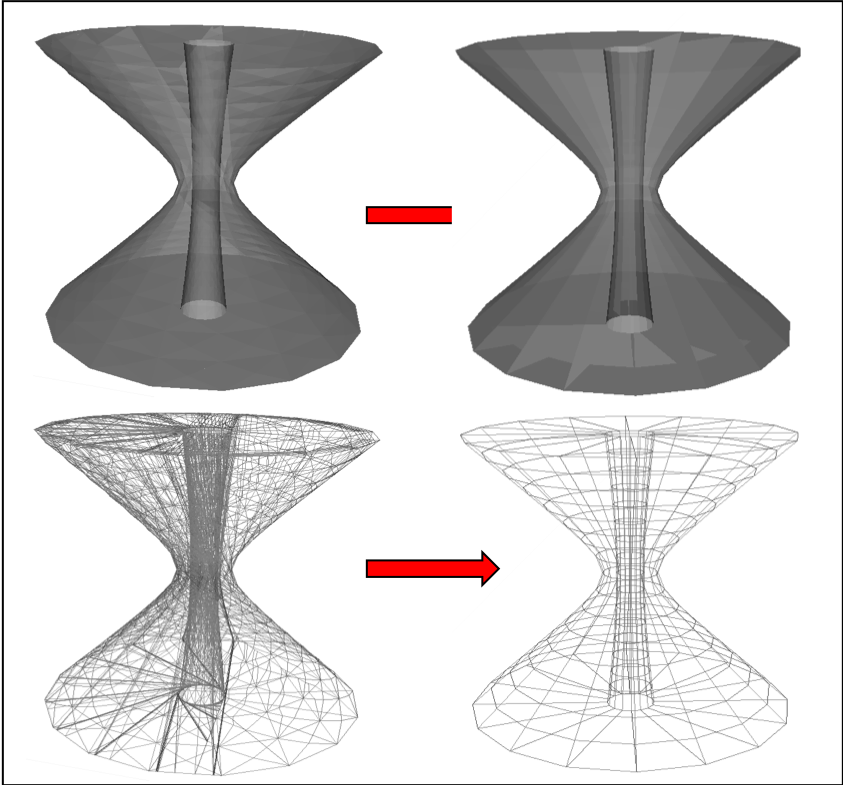
\includegraphics[height=0.9\linewidth]{Images//Meshes//hyperboloid.png}
  \captionof{figure}{ }
  \label{fig:test1}
\end{minipage}%
\begin{minipage}{.3\textwidth}
  \centering
  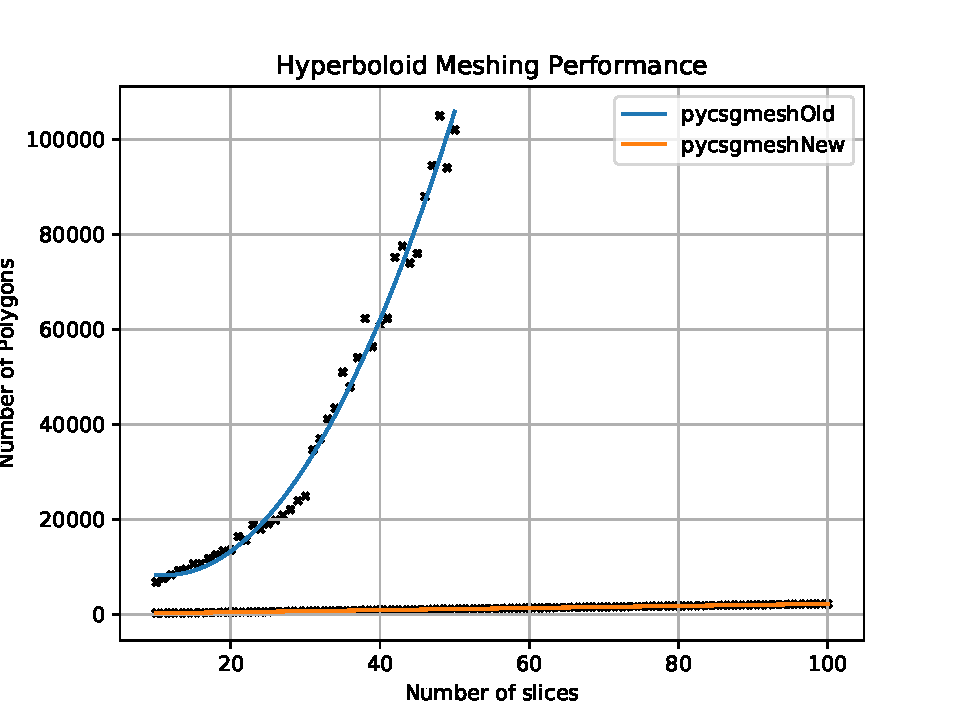
\includegraphics[scale=0.35]{Images//Quad_fits//Hyperboloid_quad.pdf}
  \captionof{figure}{ }
  \label{fig:test2}
\end{minipage}%
\end{figure}

\newpage
\subsubsection{Orb}

\begin{figure}[h!]
\centering
\begin{minipage}{.2\textwidth}
  \centering
  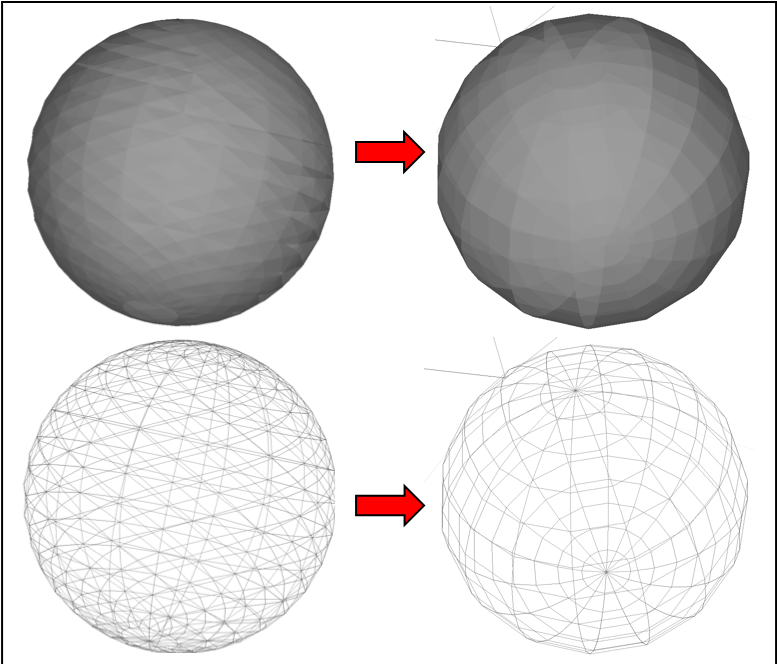
\includegraphics[height=0.8\linewidth]{Images//Meshes//orb.png}
  \captionof{figure}{ }
  \label{fig:test1}
\end{minipage}%
\begin{minipage}{.3\textwidth}
  \centering
  \includegraphics[scale=0.35]{Images//Quad_fits//orb_quad.pdf}
  \captionof{figure}{ }
  \label{fig:test2}
\end{minipage}%
\end{figure}


\subsubsection{Paraboloid}

\begin{figure}[h!]
\centering
\begin{minipage}{.2\textwidth}
  \centering
  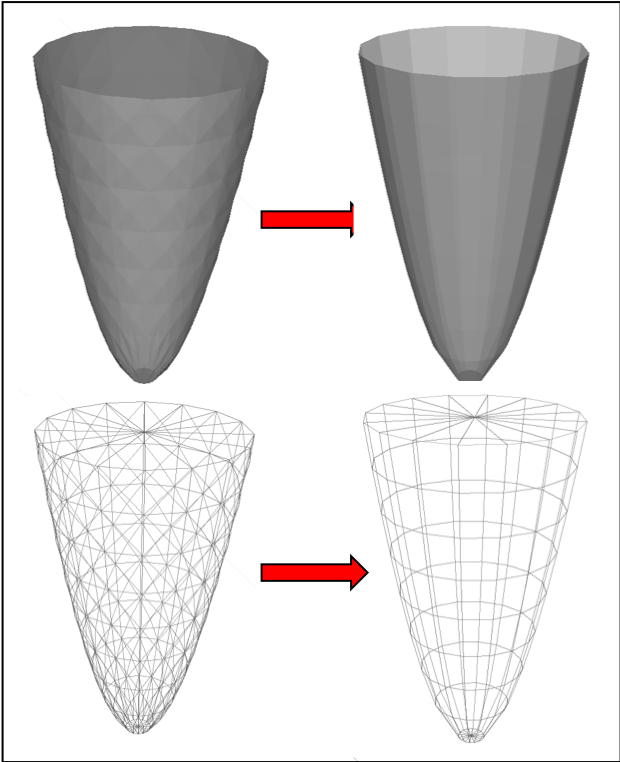
\includegraphics[height=1\linewidth]{Images//Meshes//paraboloid.png}
  \captionof{figure}{ }
  \label{fig:test1}
\end{minipage}%
\begin{minipage}{.3\textwidth}
  \centering
  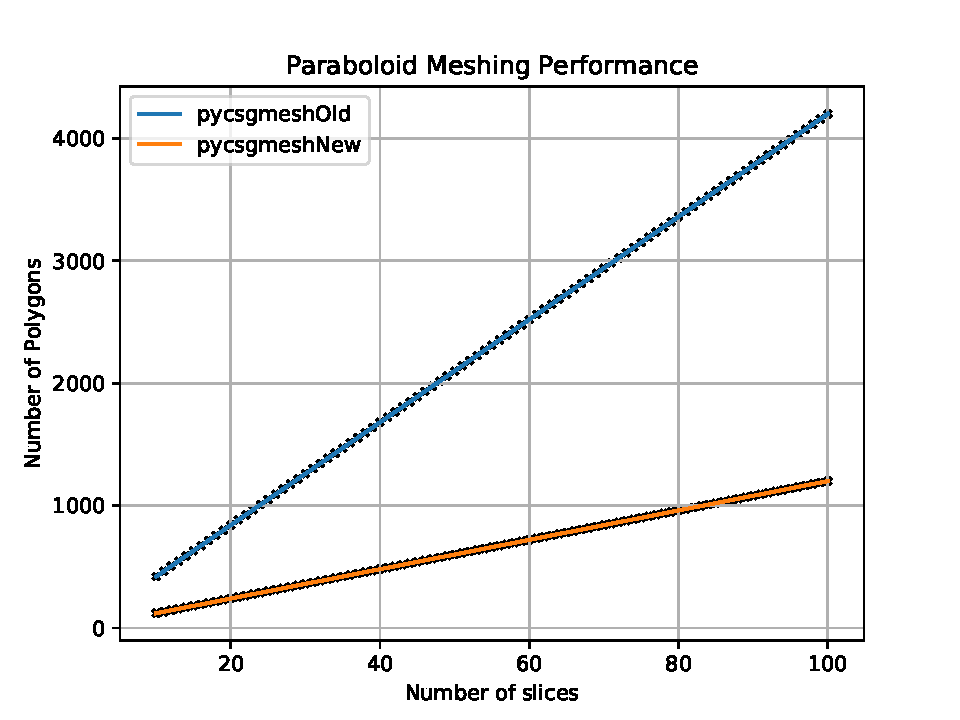
\includegraphics[scale=0.35]{Images//Quad_fits//Paraboloid_quad.pdf}
  \captionof{figure}{ }
  \label{fig:test2}
\end{minipage}%
\end{figure}


\subsubsection{Polycone}
\begin{figure}[h!]
\centering
\begin{minipage}{.2\textwidth}
  \centering
  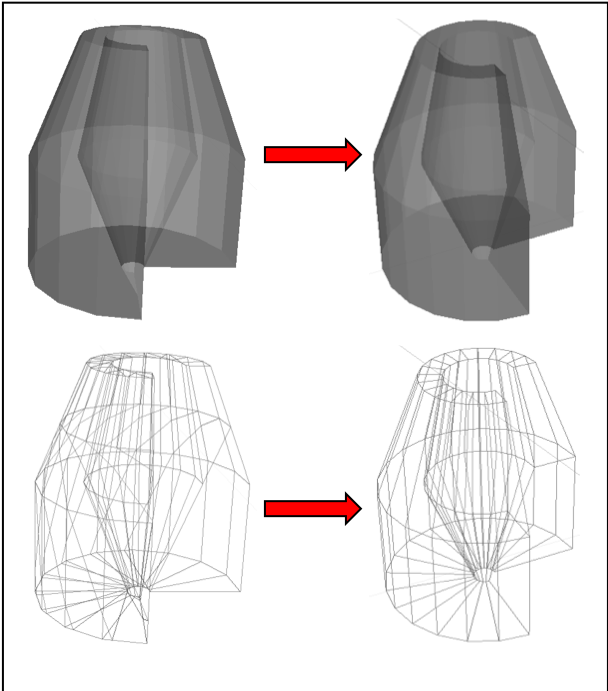
\includegraphics[height=1\linewidth]{Images//Meshes//polycone.png}
  \captionof{figure}{ }
  \label{fig:test1}
\end{minipage}%
\begin{minipage}{.3\textwidth}
  \centering
  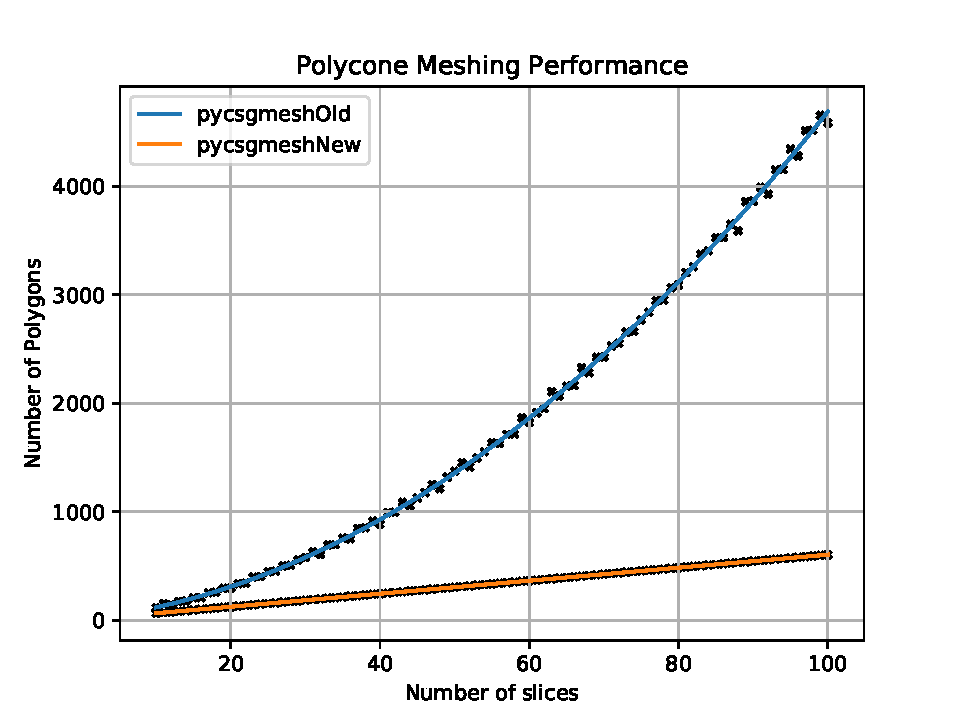
\includegraphics[scale=0.35]{Images//Quad_fits//Polycone_quad.pdf}
  \captionof{figure}{ }
  \label{fig:test2}
\end{minipage}%
\end{figure}

\newpage
\subsubsection{Sphere}
\begin{figure}[h!]
\centering
\begin{minipage}{.2\textwidth}
  \centering
  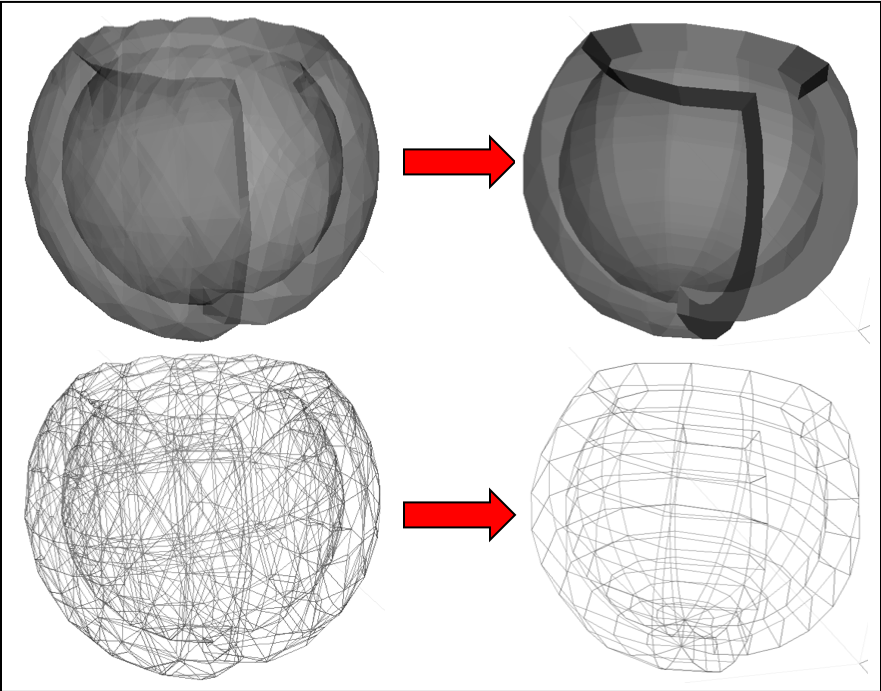
\includegraphics[height=0.75\linewidth]{Images//Meshes//sphere.png}
  \captionof{figure}{ }
  \label{fig:test1}
\end{minipage}%
\begin{minipage}{.3\textwidth}
  \centering
  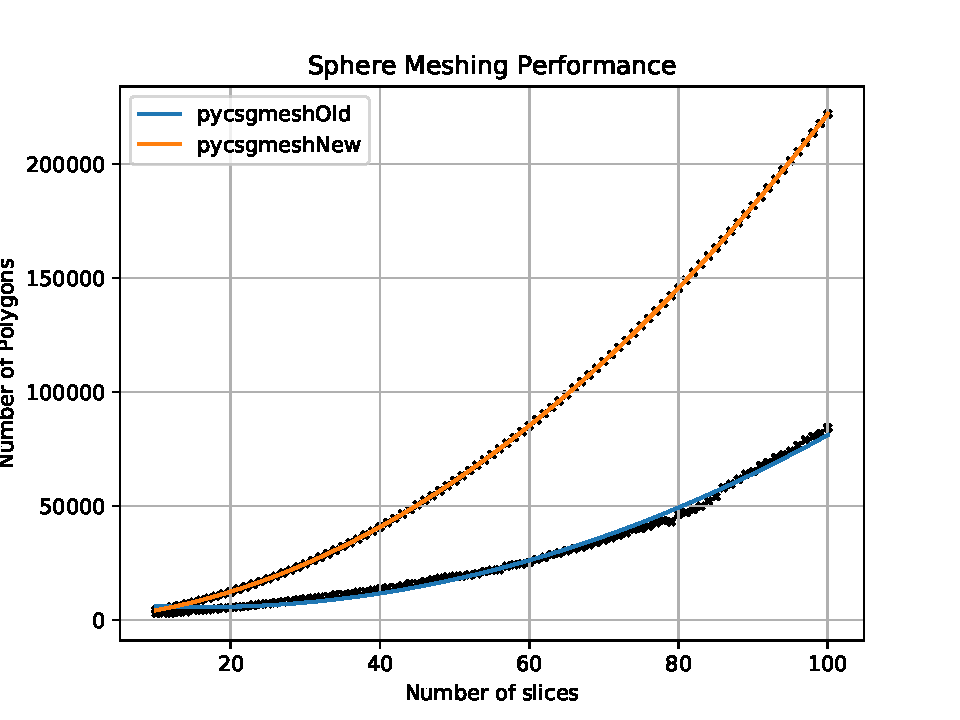
\includegraphics[scale=0.35]{Images//Quad_fits//Sphere_quad.pdf}
  \captionof{figure}{ }
  \label{fig:test2}
\end{minipage}%
\end{figure}

\subsubsection{Torus}

\begin{figure}[h!]
\centering
\begin{minipage}{.2\textwidth}
  \centering
  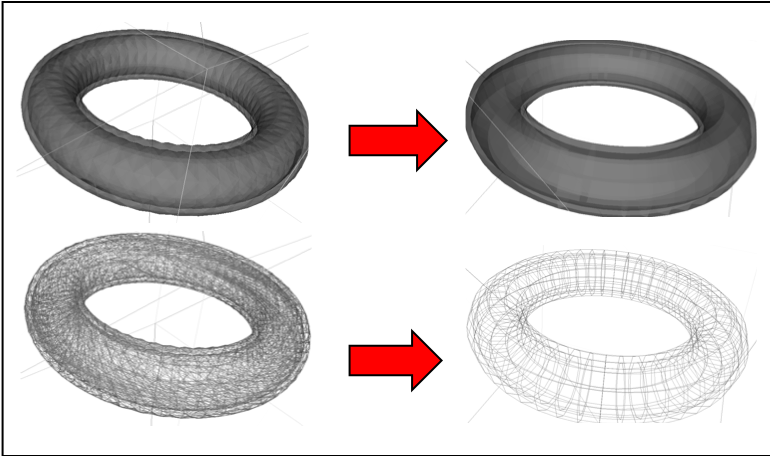
\includegraphics[height=0.5\linewidth]{Images//Meshes//torus.png}
  \captionof{figure}{ }
  \label{fig:test1}
\end{minipage}%
\begin{minipage}{.3\textwidth}
  \centering
  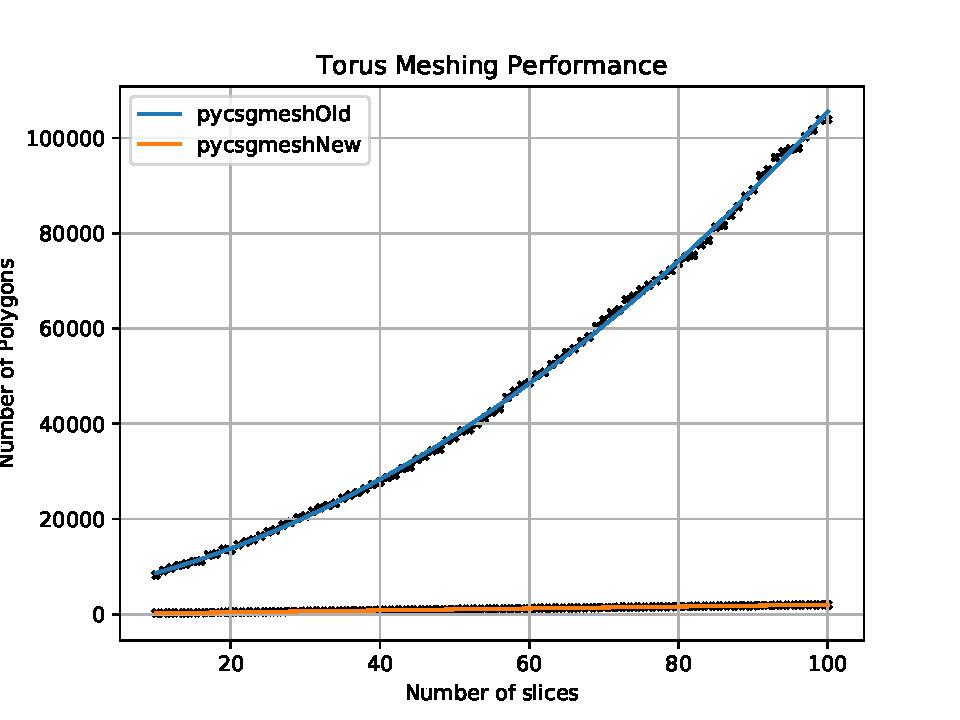
\includegraphics[scale=0.35]{Images//Quad_fits//Torus_quad.pdf}
  \captionof{figure}{ }
  \label{fig:test2}
\end{minipage}%
\end{figure}

\subsubsection{Tubs}

\begin{figure}[h!]
\centering
\begin{minipage}{.2\textwidth}
  \centering
  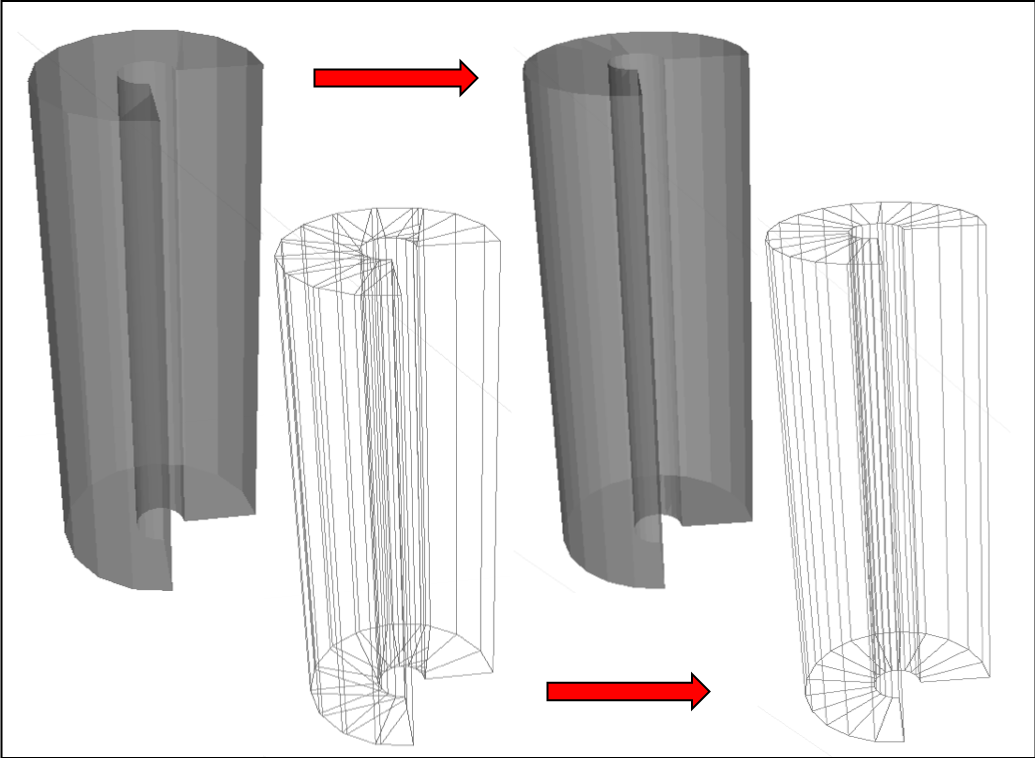
\includegraphics[height=0.7\linewidth]{Images//Meshes//tubs.png}
  \captionof{figure}{ }
  \label{fig:test1}
\end{minipage}%
\begin{minipage}{.3\textwidth}
  \centering
  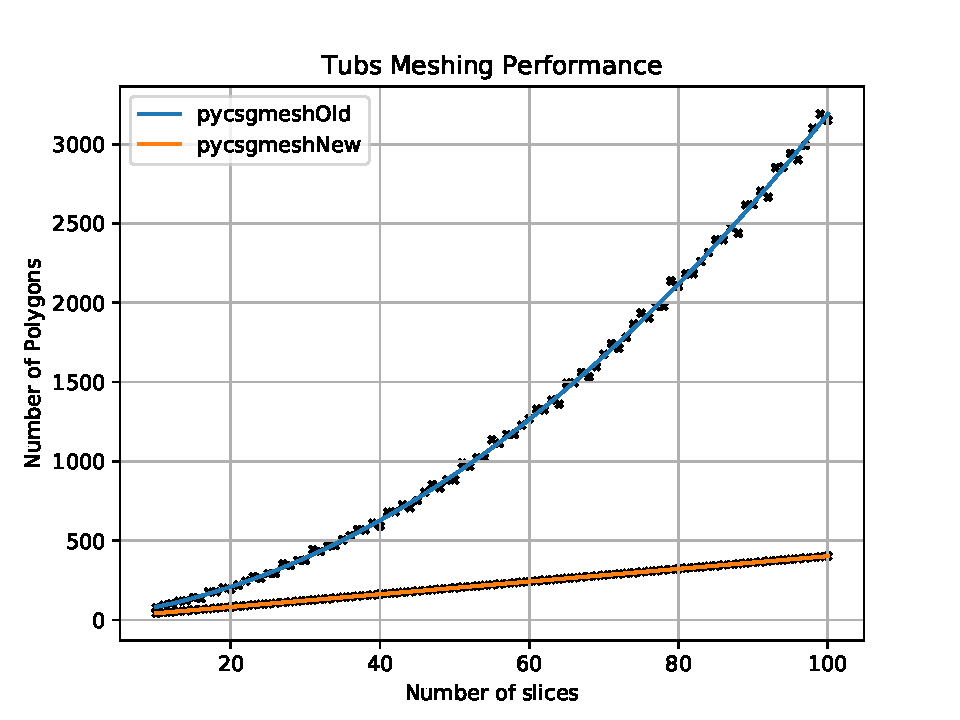
\includegraphics[scale=0.35]{Images//Quad_fits//Tubs_quad.pdf}
  \captionof{figure}{ }
  \label{fig:test2}
\end{minipage}%
\end{figure}

\endgroup
% ------------------------------------------------------------------------------------------------------------------------------

\onecolumn
\newpage
\begin{thebibliography}{1}
	\bibitem{}
		BDSIM Manual\\
		\url{http://www.pp.rhul.ac.uk/bdsim/manual/}
		
	\bibitem{}
		Pg4ometry BitBucket\\
		\url{https://bitbucket.org/jairhul/pyg4ometry/src/}
		
	\bibitem{}
	Geant4 Solids\\
	\url{http://geant4-userdoc.web.cern.ch/geant4-userdoc/UsersGuides/ForApplicationDeveloper/html/Detector/Geometry/geomSolids.html}
	
	\bibitem{}
	JAI\\
	\url{https://www.adams-institute.ac.uk/}
		
		

\end{thebibliography}

\end{document}